\subsection{Differential gears}

Differential gears are used to reduce slipping between opposite wheels when the vehicle is turning. The system can not avoid slipping under the tracks because they are too long, they will rotate at least around the center of the track. However, using differential gears will help control the course of the vehicle by braking one of the tracks and transfering some of it's power to the other track.\\

The system of differential gears is simple. As seen on \figref{diffGearLight}, the power is transmitted from the pinion gear(not represented on this picture) to the spider gear in green fixed on the ring gear in blue. Only the spider gear is connected to the side gears in pink and yellow, fixed to the wheels.
When the ring gear is turning but the spider gear does not spin, both side gear turn the same speed, but if one side gear is blocked, the spider gear will spin,  and the other side gear will turn faster.\\

\begin{figure}[H]
	\centering
	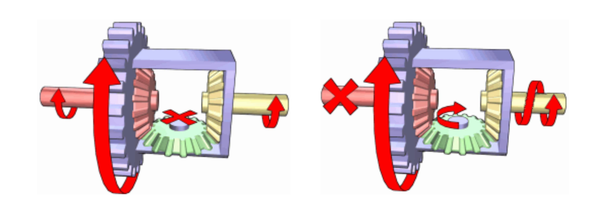
\includegraphics[scale=0.13]{figures/diffGearLight}
	\caption{Transfer of the power to the side gear when the spider gear is blocked vs when it spins}
	\label{diffGearLight}
\end{figure}

There are usually two spider gears for more reliability and solidity, and the ring gear is set in motion by the pinion gear as seen on \figref{diffGearFull}.\\

\begin{figure}[H]
	\centering
	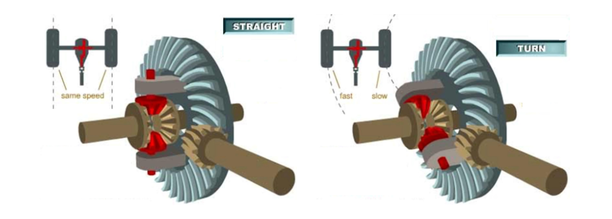
\includegraphics[scale=0.14]{figures/diffGearFull}
	\caption{Description of the differential system going straight vs turning}
	\label{diffGearFull}
\end{figure}

This is the element the servo is using when braking one track, allowing the other track to turn still.\\